\documentclass[aspectratio=169]{beamer}
\usetheme{Madrid}
\usecolortheme{default}

\usepackage{booktabs}
\usepackage{amsmath}
\usepackage{graphicx}
\usepackage{tikz}
\usepackage{xcolor}

% Custom colors
\definecolor{maincolor}{RGB}{0,102,204}
\definecolor{alertcolor}{RGB}{204,0,0}
\definecolor{goodcolor}{RGB}{0,153,0}

\setbeamercolor{structure}{fg=maincolor}
\setbeamercolor{alerted text}{fg=alertcolor}

% Remove navigation symbols
\setbeamertemplate{navigation symbols}{}

% Add frame numbers
\setbeamertemplate{footline}[frame number]

\title{The Autocorrelation Mirage}
\subtitle{Pseudoreplication Dominates Leakage in Rare-Event Panel Forecasting}
\author{Behnaz Moradi-Jamei \and Heman Shakeri}
\institute{James Madison University \and University of Virginia}
\date{\today}

\begin{document}

% Title slide
\begin{frame}
\titlepage
\end{frame}

% Outline
\begin{frame}{Outline}
\tableofcontents
\end{frame}

\section{The Problem}

\begin{frame}{Rare-Event Forecasting Challenge}
\begin{columns}[T]
\column{0.5\textwidth}
\textbf{The Setting:}
\begin{itemize}
\item Coups, equipment failures, patient deterioration
\item $n \approx 20$--50 episodes
\item $p \approx 10$--20 features
\item \alert{EPV $< 1.0$}
\end{itemize}

\vspace{1em}
\textbf{The Problem:}
\begin{itemize}
\item Far below EPV $> 10$--20 required for stable inference
\item Can't train reliable models
\end{itemize}

\column{0.5\textwidth}
\begin{center}
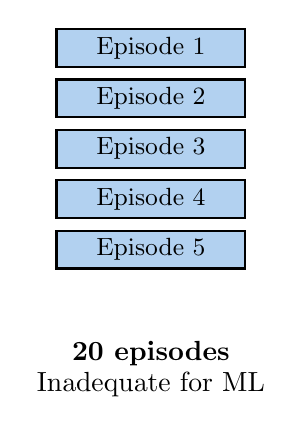
\begin{tikzpicture}[scale=0.8]
% Draw crisis episodes as blocks
\foreach \i in {1,...,5} {
    \draw[fill=maincolor!30, thick] (0, -\i*0.8) rectangle (3, -\i*0.8+0.6);
    \node at (1.5, -\i*0.8+0.3) {\small Episode \i};
}
\node[below] at (1.5, -5) {\textbf{20 episodes}};
\node[below] at (1.5, -5.5) {\alert{Inadequate for ML}};
\end{tikzpicture}
\end{center}
\end{columns}
\end{frame}

\begin{frame}{The Common Solution: Panel Expansion}
\begin{center}
\textbf{Transform each episode into daily observations}

\vspace{1em}
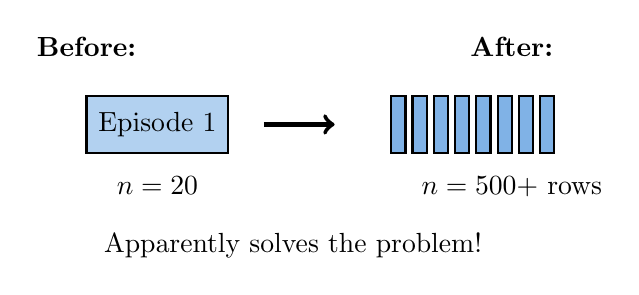
\begin{tikzpicture}[scale=0.9]
% Before
\node at (0, 2) {\textbf{Before:}};
\draw[fill=maincolor!30, thick] (0, 0.5) rectangle (2, 1.3);
\node at (1, 0.9) {Episode 1};
\node[below] at (1, 0.3) {$n = 20$};

% Arrow
\draw[->, ultra thick] (2.5, 0.9) -- (3.5, 0.9);

% After
\node at (6, 2) {\textbf{After:}};
\foreach \i in {1,...,8} {
    \draw[fill=maincolor!50, thick] (4+\i*0.3, 0.5) rectangle (4.2+\i*0.3, 1.3);
}
\node[below] at (6, 0.3) {$n = 500+$ rows};

\node[below, align=center] at (3, -0.5) {
    \alert{Apparently solves the problem!}
};
\end{tikzpicture}
\end{center}

\vspace{1em}
\begin{center}
\Large But does it really?
\end{center}
\end{frame}

\section{Two Failure Modes}

\begin{frame}{Two Silent Failures}
\begin{columns}[T]
\column{0.48\textwidth}
\begin{block}{Failure \#1: Label Leakage}
Features that depend on $T_e$ create target leakage
\[X_{e,t} = f(T_e - t) + \epsilon\]
\textbf{Known problem} (Kaufman et al. 2012)
\end{block}

\column{0.48\textwidth}
\begin{block}{Failure \#2: Pseudoreplication}
Row-wise CV treats correlated observations as independent
\[\text{Same episode in train \& test}\]
\textbf{Our focus:} More dangerous than leakage!
\end{block}
\end{columns}

\vspace{2em}
\begin{center}
\Large\alert{Which is the greater threat?}
\end{center}
\end{frame}

\begin{frame}{Research Question}
\begin{center}
\LARGE
\textbf{In panel-expanded rare-event forecasting,}\\[0.5em]
\textbf{which failure mode dominates?}

\vspace{2em}
\large
\structure{Spoiler:} It's not the one everyone worries about...
\end{center}
\end{frame}

\section{Episode Memorization}

\begin{frame}{The Mechanism: Episode Memorization}
\textbf{What standard K-Fold CV does:}
\begin{enumerate}
\item Randomly assigns \alert{rows} to folds
\item Episode $e$ appears in \alert{both} training and test
\item Consecutive observations $X_{e,t}$ and $X_{e,t+1}$ highly correlated
\end{enumerate}

\vspace{1em}
\textbf{What the model learns:}
\begin{itemize}
\item Not: ``What patterns precede events?''
\item But: \alert{``Which episode does this belong to?''}
\item Identity inference → pattern matching → artificial accuracy
\end{itemize}

\vspace{1em}
\begin{center}
\tikz{
    \node[draw, fill=alertcolor!20, rounded corners, text width=0.7\textwidth, align=center] {
        \textbf{Forecasting} (extrapolation to new episodes)\\
        transforms into\\
        \textbf{Interpolation} (pattern-matching within known episodes)
    };
}
\end{center}
\end{frame}

\begin{frame}{Visualizing the Problem}
\begin{columns}[T]
\column{0.48\textwidth}
\textbf{Standard K-Fold (WRONG):}
\begin{center}
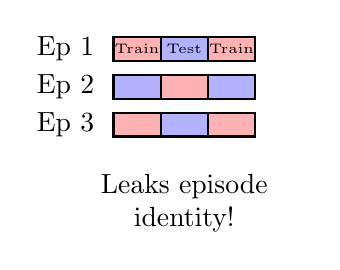
\begin{tikzpicture}[scale=0.6]
% Episode 1 split across folds
\draw[fill=red!30, thick] (0, 3) rectangle (1, 3.5);
\node at (0.5, 3.25) {\tiny Train};
\draw[fill=blue!30, thick] (1, 3) rectangle (2, 3.5);
\node at (1.5, 3.25) {\tiny Test};
\draw[fill=red!30, thick] (2, 3) rectangle (3, 3.5);
\node at (2.5, 3.25) {\tiny Train};
\node[left] at (-0.2, 3.25) {Ep 1};

% Episode 2 split
\draw[fill=blue!30, thick] (0, 2.2) rectangle (1, 2.7);
\draw[fill=red!30, thick] (1, 2.2) rectangle (2, 2.7);
\draw[fill=blue!30, thick] (2, 2.2) rectangle (3, 2.7);
\node[left] at (-0.2, 2.45) {Ep 2};

% Episode 3 split
\draw[fill=red!30, thick] (0, 1.4) rectangle (1, 1.9);
\draw[fill=blue!30, thick] (1, 1.4) rectangle (2, 1.9);
\draw[fill=red!30, thick] (2, 1.4) rectangle (3, 1.9);
\node[left] at (-0.2, 1.65) {Ep 3};

\node[below, align=center, text width=3cm] at (1.5, 0.8) {
    \alert{Leaks episode identity!}
};
\end{tikzpicture}
\end{center}

\column{0.48\textwidth}
\textbf{Episode-Grouped (CORRECT):}
\begin{center}
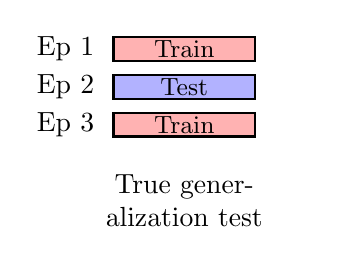
\begin{tikzpicture}[scale=0.6]
% Episode 1 all in train
\draw[fill=red!30, thick] (0, 3) rectangle (3, 3.5);
\node at (1.5, 3.25) {\small Train};
\node[left] at (-0.2, 3.25) {Ep 1};

% Episode 2 all in test
\draw[fill=blue!30, thick] (0, 2.2) rectangle (3, 2.7);
\node at (1.5, 2.45) {\small Test};
\node[left] at (-0.2, 2.45) {Ep 2};

% Episode 3 all in train
\draw[fill=red!30, thick] (0, 1.4) rectangle (3, 1.9);
\node at (1.5, 1.65) {\small Train};
\node[left] at (-0.2, 1.65) {Ep 3};

\node[below, align=center, text width=3cm] at (1.5, 0.8) {
    \structure{True generalization test}
};
\end{tikzpicture}
\end{center}
\end{columns}
\end{frame}

\section{Simulation}

\begin{frame}{Simulation Setup}
\textbf{Goal:} Isolate each failure mode independently

\vspace{0.5em}
\textbf{Design:} $E = 30$ episodes with:
\begin{itemize}
\item Episode effects: $\alpha_e \sim \mathcal{N}(0, 0.5)$
\item AR(1) latent process: $Z_{e,t} = 0.7 Z_{e,t-1} + \epsilon_t$
\item Hazard: $h_{e,t} = \text{logit}^{-1}(-3 + \alpha_e + 0.15 Z_{e,t})$
\item \structure{Key:} The $-3$ intercept produces \alert{$\sim$5\% event rate} (truly rare!)
\item Features: \textbf{strictly causal} (from $Z_{e,<t}$ only)
\item Label: $Y_{e,t} = \mathbf{1}\{t < T_e \leq t+14\}$
\end{itemize}

\vspace{0.5em}
\textbf{Four Conditions:}
\begin{enumerate}
\item Leak-free + Grouped CV \hfill (baseline)
\item Leak-free + Random CV \hfill \alert{(pseudoreplication test)}
\item Normalization leak + Grouped CV
\item Explicit $T_e - t$ leak + Grouped CV \hfill \alert{(leakage test)}
\end{enumerate}
\end{frame}

\section{Main Result}

\begin{frame}{The Main Finding}
\begin{center}
\LARGE\structure{Pseudoreplication > Leakage}

\vspace{2em}
\begin{tabular}{lcc}
\toprule
\textbf{Failure Mode} & \textbf{AUC Inflation} & \textbf{Relative} \\
\midrule
\alert{Pseudoreplication} & 0.56 → 0.86 & \alert{+54\%} \\
Explicit Leakage & 0.56 → 0.77 & +39\% \\
\bottomrule
\end{tabular}

\vspace{2em}
\Large
\alert{The standard tool is more dangerous}\\
\alert{than the worst feature-engineering error!}
\end{center}
\end{frame}

\begin{frame}{Detailed Results}
\begin{table}
\centering
\small
\begin{tabular}{lccc}
\toprule
\textbf{Condition} & \textbf{AUC} & \textbf{Brier} & \textbf{Inflation} \\
\midrule
Leak-Free + Grouped CV & 0.56 $\pm$ 0.07 & 0.29 $\pm$ 0.05 & baseline \\
\rowcolor{red!10}
Leak-Free + Random CV & \textbf{0.86 $\pm$ 0.04} & 0.15 $\pm$ 0.02 & \alert{+54\%} \\
Norm. Leak + Grouped & 0.56 $\pm$ 0.07 & 0.29 $\pm$ 0.05 & +0\%$^\dagger$ \\
Explicit Leak + Grouped & 0.77 $\pm$ 0.04 & 0.16 $\pm$ 0.03 & +39\% \\
\bottomrule
\end{tabular}
\end{table}

\vspace{0.5em}
\footnotesize
$^\dagger$Normalization leak requires pre-existing trends; our AR(1) features are stationary (conservative design)

\vspace{1em}
\textbf{Key insight:} Autocorrelation alone (no trends, no leakage) destroys validity
\end{frame}

\begin{frame}{Why Pseudoreplication Dominates}
\begin{columns}[T]
\column{0.48\textwidth}
\textbf{Leakage:}
\begin{itemize}
\item Requires specific conditions
\item Explicit $T_e - t$ features
\item OR trending features + global normalization
\item \structure{Visible in code review}
\end{itemize}

\column{0.48\textwidth}
\textbf{Pseudoreplication:}
\begin{itemize}
\item Requires \alert{only default KFold}
\item Single line of code everyone uses
\item \alert{Invisible and ubiquitous}
\item \alert{Activated by default}
\end{itemize}
\end{columns}

\vspace{2em}
\begin{center}
\tikz{
    \node[draw, fill=alertcolor!20, rounded corners, text width=0.8\textwidth, align=center, thick] {
        \textbf{Asymmetry:} Leakage is rare and detectable.\\
        Pseudoreplication is \alert{everywhere} and invisible.
    };
}
\end{center}
\end{frame}

\begin{frame}{Performance Decouples from Sample Size}
\begin{center}
\structure{Under random CV, performance ignores effective $n$:}

\vspace{0.5em}

\includegraphics[width=0.7\textwidth]{figs/figure1_simulation_results.png}

\vspace{0.5em}
\small
Panel D shows: Model achieves AUC $> 0.8$ even when $n_{\text{eff}} < 50$\\
\alert{→ Exploiting autocorrelation artifact, not learning generalizable signal}
\end{center}
\end{frame}

\section{The Solution}

\begin{frame}{The $\Delta_{\text{CV}}$ Diagnostic}
\textbf{Simple check for episode memorization:}
\[\Delta_{\text{CV}} := \widehat{\text{AUC}}_{\text{random}} - \widehat{\text{AUC}}_{\text{grouped}}\]

\vspace{1em}
\textbf{Interpretation:}
\begin{itemize}
\item $\Delta_{\text{CV}} < 0.05$: Model is okay
\item $\Delta_{\text{CV}} > 0.05$: \alert{Model relies on episode memorization}
\item $\Delta_{\text{CV}} > 0.10$: \alert{\textbf{Severe problem}}
\end{itemize}

\vspace{1em}
\textbf{In our simulation:} $\Delta_{\text{CV}} = 0.30$ (catastrophic!)

\vspace{1em}
\structure{Requires no new data—just re-run with GroupKFold}
\end{frame}

\begin{frame}{Corrected Protocol}
\begin{enumerate}
\item \textbf{Preprocessing:}
\begin{itemize}
\item Fit transformations on training fold only
\item Forward-fill imputation (not mean)
\item Trailing windows (not centered)
\end{itemize}

\vspace{0.5em}
\item \textbf{Evaluation:}
\begin{itemize}
\item Use \texttt{GroupKFold} with \texttt{groups=episode\_id}
\item \alert{Never split episodes across folds}
\end{itemize}

\vspace{0.5em}
\item \textbf{Reporting:}
\begin{itemize}
\item Report $\Delta_{\text{CV}}$ alongside AUC
\item Report $n_{\text{eff}}$ (effective sample size)
\item Brier Score and Log Loss as primary metrics
\end{itemize}
\end{enumerate}
\end{frame}

\begin{frame}{Red Flags}
\begin{center}
\Large\alert{Warning signs that should trigger audits:}

\vspace{1em}
\begin{tabular}{ll}
\toprule
\textbf{Metric} & \textbf{Threshold} \\
\midrule
AUC & $> 0.85$ with $E < 50$ episodes \\
$\Delta_{\text{CV}}$ & $> 0.10$ \\
Brier Score & $< 0.10$ on imbalanced data \\
\bottomrule
\end{tabular}

\vspace{2em}
\structure{If you see performance this good on rare events...}\\
\structure{...it's probably too good to be true!}
\end{center}
\end{frame}

\section{Implications}

\begin{frame}{Affected Domains}
\textbf{This pathology affects any field using panel-expanded forecasting:}

\vspace{0.5em}
\begin{columns}[T]
\column{0.48\textwidth}
\begin{itemize}
\item \structure{Geopolitics:} Conflict forecasting, coups
\item \structure{Healthcare:} Clinical deterioration, mortality
\item \structure{Engineering:} Predictive maintenance, equipment failure
\end{itemize}

\column{0.48\textwidth}
\begin{itemize}
\item \structure{Business:} Customer churn, default prediction
\item \structure{Finance:} Credit events, bankruptcy
\item \structure{Any rare event} expanded into daily/hourly panels
\end{itemize}
\end{columns}

\vspace{1em}
\begin{center}
\tikz{
    \node[draw, fill=maincolor!20, rounded corners, text width=0.9\textwidth, align=center, thick] {
        \textbf{Call for Action:} Retrospective audits of published claims\\
        in rare-event forecasting using panel data
    };
}
\end{center}
\end{frame}

\begin{frame}{Relation to Prior Work}
\textbf{We unify three research streams:}

\vspace{0.5em}
\begin{enumerate}
\item \textbf{Kaufman et al. (2012):} Leakage formalization, learn-predict separation
\begin{itemize}
\item But: focused on i.i.d. data, explicit violations
\end{itemize}

\vspace{0.3em}
\item \textbf{Roberts et al. (2017):} Block CV for structured data
\begin{itemize}
\item But: spatial dependence in ecology, not temporal panels
\end{itemize}

\vspace{0.3em}
\item \textbf{Hurlbert (1984):} Pseudoreplication in experiments
\begin{itemize}
\item But: experimental design, not ML evaluation
\end{itemize}
\end{enumerate}

\vspace{1em}
\structure{Our contribution:} Pseudoreplication \alert{dominates} in panel forecasting + $\Delta_{\text{CV}}$ diagnostic
\end{frame}

\section{Conclusion}

\begin{frame}{Key Takeaways}
\begin{enumerate}
\item Panel expansion creates value \alert{only if evaluation respects episode boundaries}

\vspace{0.5em}
\item Standard K-Fold CV—\alert{the default in Scikit-Learn}—violates this

\vspace{0.5em}
\item Result: \alert{Episode memorization} inflates AUC by 54\%

\vspace{0.5em}
\item This \alert{exceeds explicit leakage} (+39\%)

\vspace{0.5em}
\item The $\Delta_{\text{CV}}$ diagnostic provides a simple check

\vspace{0.5em}
\item \textbf{Action:} Use \texttt{GroupKFold}, report $\Delta_{\text{CV}}$ and $n_{\text{eff}}$
\end{enumerate}
\end{frame}

\begin{frame}{The Bottom Line}
\begin{center}
\LARGE
\alert{The standard tool is more dangerous}\\[0.3em]
\alert{than the worst feature-engineering error}

\vspace{2em}
\Large
\structure{Pseudoreplication is:}
\begin{itemize}
\item Invisible
\item Ubiquitous  
\item Activated by default
\item More impactful than explicit leakage
\end{itemize}

\vspace{1em}
\normalsize
\textbf{For reviewers:} Demand grouped CV, $\Delta_{\text{CV}}$ reporting, and $n_{\text{eff}}$ disclosure
\end{center}
\end{frame}

\begin{frame}[standout]
\begin{center}
\LARGE
Thank you!

\vspace{2em}
\normalsize
\textbf{Behnaz Moradi-Jamei}\\
moradibx@jmu.edu

\vspace{0.5em}
\textbf{Heman Shakeri}\\
hs@virginia.edu

\vspace{2em}
\structure{Code \& Materials:}\\
\texttt{github.com/[your-repo]}
\end{center}
\end{frame}

\appendix

\begin{frame}[allowframebreaks]{Backup: Effective Sample Size}
\textbf{Under intraclass correlation $\rho$ with $m$ observations per episode:}
\[n_{\text{eff}} = \frac{n}{1 + (m-1)\rho}\]

\vspace{1em}
\textbf{Example:} $n = 600$, $m = 20$, $\rho = 0.5$
\[n_{\text{eff}} = \frac{600}{1 + 19 \times 0.5} = \frac{600}{10.5} \approx 55\]

\vspace{1em}
\alert{10× reduction in effective sample size!}

\vspace{1em}
But pseudoreplication inflation is \textbf{not} just a sample-size effect—even with $n_{\text{eff}} < 20$, random CV achieves AUC $> 0.8$.
\end{frame}

\begin{frame}[allowframebreaks]{Backup: Why -3 Intercept?}
\textbf{Hazard function:} $h_{e,t} = \text{logit}^{-1}(-3 + \alpha_e + 0.15 Z_{e,t})$

\vspace{0.5em}
\textbf{Why the -3?}
\begin{itemize}
\item For average episode ($\alpha_e = 0$, $Z_{e,t} = 0$):
\[h_t = \text{logit}^{-1}(-3) = \frac{1}{1 + e^3} \approx 0.047 \approx 5\%\]

\item Creates \alert{truly rare events} (5\% base rate)
\item Matches empirical geopolitical event frequencies
\item Produces severe EPV constraint (EPV $< 5$)
\end{itemize}

\vspace{0.5em}
\textbf{Without -3:} Events would occur $\sim$50\% of the time (not rare!)
\end{frame}

\end{document}
